\section{Filtertheorie \formelbuch{301} \tiny{$Revision: 996 $}}
\begin{tabular}{ll}
\parbox{12cm}{
	Man unterscheidet die Filtertypen grundsätzlich zwischen
	Tief-, Hoch- und Bandpässen sowie Bandsperren.
	
	\subsection{Toleranzschema \formelbuch{307}}
	Im Durchlassbereich (DB) bestimmt der Stempel die maximal zul"assige D"ampfung
	$A_{\max}$; im Sperrbereich (SB) bestimmt die Matrize die minimal n"otige
	D"ampfung $A_{\min}$.
	}
& \parbox{6cm}{
	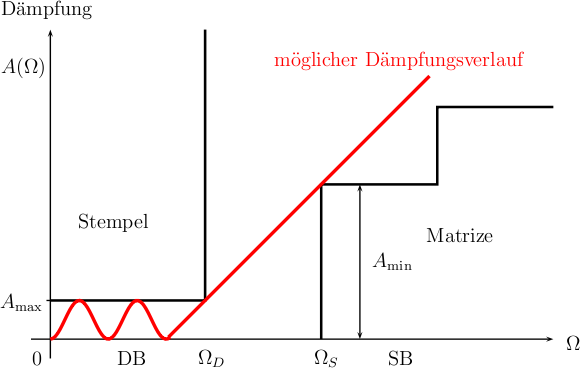
\includegraphics[width=6cm]{./images/filter-toleranzschema.png}}
\end{tabular}

\subsection{Realisation analoger Filter}
\subsubsection{Allgemeines Vorgehen}
\begin{itemize}
  \item[1.] Frequenznormierung durchführen
  \item[2.] Normierten Tiefpass bestimmen (Filter nach Tiefpass transformieren)
  \item[3.] Art der Approximation wählen: Butterworth, Tschebyscheff (I, II),
  Cauer, Bessel, Gauss, \ldots
  \item[4.] Bestimmung der Ordnung mit Nomogrammen \formelbuch{404}, Matlab
	\matlab{buttord, cheb1ord, cheb2ord, ellipord} oder Formeln
  \item[5.] Normierte TP-UTF aus Tabellen entnehmen \& entnormieren
  \item[6.] Aus Tabelle \formelbuch{420} L und C-Werte für Tiefpass heraus lesen
  \& entnormieren
  \item[7.] Filter von Tiefpass zum gesuchten Filter rücktransformieren
\end{itemize}


\subsubsection{Frequenznormierung \formelbuch{308}}
\begin{tabular}{ll}
\parbox{6cm}{
	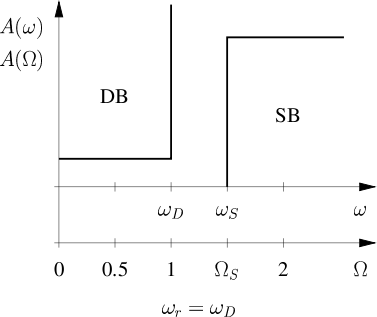
\includegraphics[width=5cm]{./images/filter-freqnormierung.png}}
& \parbox{12cm}{
	\textbf{Normierung} \\
	$S=\frac{s}{\omega_{r}} \hspace{2cm} \Omega=\frac{\omega}{\omega_{r}} 
\hspace{2cm} \sigma'=\frac{\sigma}{\omega_{r}}$\\ 

	Bei Bandpässen \& -sperren: $\omega_r = \sqrt{\omega_{D1} \omega_{D2}}
	\underbrace{=}_{\text{\tiny{wenn symmetrisch}}} \sqrt{\omega_{S1} \omega_{S2}}$
	\\

	Zur Entnormierung wird $\omega_{3db}$ gebraucht, daher sind diese Formeln
	dafür nicht geeignet! \\
	}
\end{tabular}

\subsubsection{Filtertransformationen \formelbuch{355}}
\begin{tabular}{|ll|l|l|}
\hline
\multicolumn{2}{|l|}{\textbf{Tiefpass-Hochpass \formelbuch{302}}}
	& \textbf{Tiefpass-Bandpass \formelbuch{304}}
	& \textbf{Tiefpass-Bandsperre \formelbuch{308}} \\ 
\multicolumn{2}{|l|}{\parbox{6cm}{
	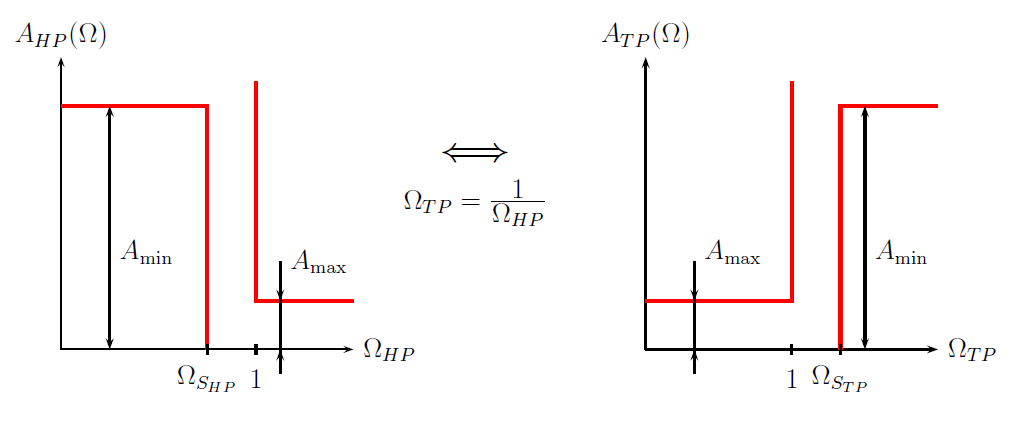
\includegraphics[width=6cm]{./images/filter-transf-tp-hp.png}
	}}
& \parbox{6cm}{
	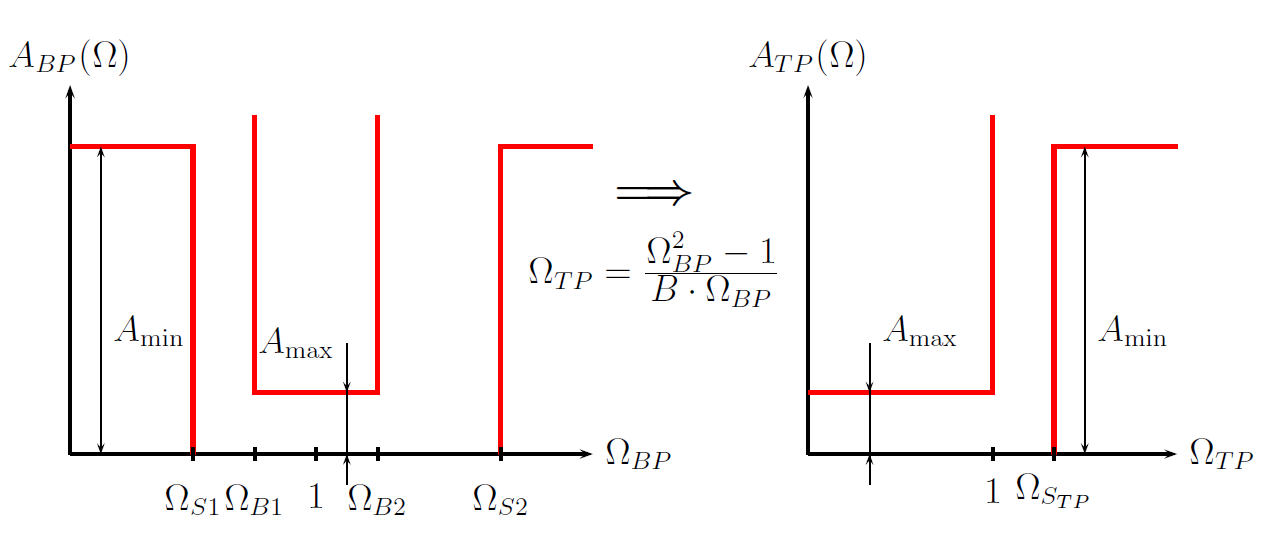
\includegraphics[width=6cm]{./images/filter-transf-tp-bp.png}
	}
& \parbox{6cm}{
	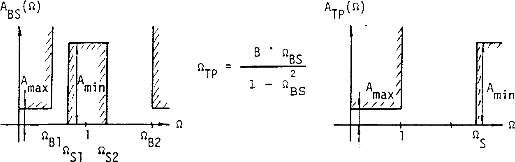
\includegraphics[width=6cm]{./images/filter-transf-tp-bs.png}
	} \\
Ordnung: 
	& $n$
	& $2n$
	& $2n$ \\
Ansatz: 
	& $S \longrightarrow \frac{1}{S}$
	& $S \longrightarrow \frac{S^{2}+1}{B\cdot S}$
	& $S \longrightarrow \frac{B\cdot S}{S^{2}+1}$ \\
UTF: 
	&$H_{HP}(S)=H_{TP}\left(\frac{1}{S}\right)$
	& $T_{BP}(S)=T_{TP}\left(\frac{S^{2}+1}{B\cdot S}\right)$
	& $T_{BS}(S)=T_{TP}\left(\frac{B\cdot S}{S^{2}+1}\right)$ \\
Norm. Frequenz: 
	& $\Omega_{S_{TP}}=\frac{1}{\Omega_{S_{HP}}}$
	& $\Omega_{S_{TP}}=\frac{\Omega_{S2}-\Omega_{S1}}{B}=
		\frac{\Omega_{S2}-\Omega_{S1}}{\Omega_{D2}-\Omega_{D1}}$
	& $\Omega_{S_{TP}}=\frac{B}{\Omega_{S2}-\Omega_{S1}}=
         \frac{\Omega_{D2}-\Omega_{D1}}{\Omega_{S2}-\Omega_{S1}}$ \\
\multicolumn{2}{|l|}{Bandbreite}
	& \multicolumn{2}{|c|}{$B = \dfrac{\omega_{D2} - \omega_{D1}}{\omega_r}$
	 } \\
\hline
\end{tabular}
\\ \\
\textbf{Direkte Substitution}\\
\renewcommand{\arraystretch}{1.5}
\begin{tabular}{|lll|}
\hline
HP-TP
	& $T_{TP}(S)=\frac{K}{b_{n}S^{n}+b_{n-1}S^{n-1}+...+b_{1}S+b_{0}}$
	& $\longrightarrow
	T_{HP}(S)=\frac{KS^{n}}{b_{0}S^{n}+b_{1}S^{n-1}+...+b_{n-1}S+b_{n}}$\\
\hline
BP-TP 1. Ordnung
	& $T_{TP}(S)=\frac{1}{S+a}$
	& $\longrightarrow 
	T_{BP}(S)=T_{TP}\left(\frac{S^{2}+1}{B\cdot S}\right)=\frac{B\cdot
	S}{S^{2}+aB\cdot S+1}$\\
BP-TP 2. Ordnung
	& $T_{TP}(S)=\frac{1}{S^{2}+aS+b}$
	& $\longrightarrow
	T_{BP}(S)=T_{TP}\left(\frac{S^{2}+1}{B\cdot S}\right)=\frac{B^{2}S^{2}}{S^{4}+aB
	S^{3}+(bB^{2}+2)S^{2}+aB\cdot S+1}$  \\
\hline 
BS-TP 1. Ordnung
	& $T_{TP}(S)=\frac{1}{S+a}$
	& $\longrightarrow
	T_{BS}(S)=T_{TP}\left(\frac{B\cdot S}{S^{2}+1}\right)=
	\frac{\frac{1}{a}(S^{2}+1)}{S^{2}+\frac{B}{a}S+1}$ \\
BS-TP 2. Ordnung
	& $T_{TP}(S)=\frac{1}{S^{2}+aS+b}$ 
	& $\longrightarrow
	T_{BS}(S) = T_{TP}\left(\frac{B\cdot S}{S^{2}+1}\right)=
	\frac{\frac{1}{b}(S^{2}+1)^{2}}{S^{4}+\frac{aB}{b}S^{3}+
	\left(\frac{B^{2}}{b}+2\right)S^{2}+\frac{aB}{b}S+1}$ \\
\hline
\end{tabular}
\renewcommand{\arraystretch}{1}


\subsubsection{Approximationsarten \formelbuch{309}}
\begin{tabular}{|p{9cm}|p{9cm}|}
\hline
\parbox{9cm}{
	\textbf{Butterworth} \formelbuch{310}
	\begin{itemize}
	 \item Amplitudengang: Gute Approximation (``maximal flach'')
	 \item Allpolfilter, Pole liegen auf Kreis mit Abstand
	 $\frac{\pi}{n}$
	 \item Gruppenlaufzeit: Leichte Überhöhung bei
	 Grenzfrequenz
	\end{itemize}
	}
& 
\parbox{9cm}{
	\textbf{Kritisch gedämpftes (Gauss)-Filter} \formelbuch{317}
	\begin{itemize}
	 \item Keine Überschwinger bei Impuls- \& Sprungantwort
	 \item Kaskadierung von wirkungsfreien RC-Filtern
	 \item Allpolfilter: Pole nur auf negativer $\sigma$-Achse
	\end{itemize}
	} \\
\hline
\parbox{9cm}{
	\textbf{Tschebyscheff I} \formelbuch{321}
	\begin{itemize}
	 \item Amplitudengang: Definierte Welligkeit im DB, steiler Übergang
	 \item Allpolfilter, wobei alle Pole auf einer Ellipse liegen
	 \item Schlechte Gruppenlaufzeit
	\end{itemize}
	}
&
 \parbox{9cm}{
	\textbf{Inverser Tschebyscheff  / Tscheby. II} \formelbuch{330}
	\begin{itemize}
	 \item Definierte Welligkeit im Sperrbereich
	 \item Flachere Gruppenlaufzeit als Tschebyscheff I
	\end{itemize}
	} \\
\hline
\parbox{6cm}{
	\textbf{Cauer} \formelbuch{333}
	\begin{itemize}
	 \item Amplitudengang: Definierte Welligkeit im SB und DB
	 \item Steilster Übergang zwischen SB und DB
	 \item bei geradem N je N konjugiert komplexe Pol- und Nullstellen
	 \item bei ungeradem N 1 reeler Pol und N-1 konjugiert komplexe Pol- Nullstellen
	\end{itemize}
	}
& 
\parbox{6cm}{
	\textbf{Bessel} \formelbuch{339}
	\begin{itemize}
	 \item Sehr linearer Phasengang $\Rightarrow$ fast konstante Gruppenlaufzeit
	 \item Flachster Übergang zw. DB und SB im Amplitudengang
	 \item Pole weit entfernt der $j \omega$-Achse
	\end{itemize}
	} \\
\hline
\end{tabular}

\subsubsection{Bestimmung der minimal nötigen Ordnung \formelbuch{???}}
\begin{tabular}{p{7cm} p{11cm}}
\parbox{6cm}{
	\textbf{Mittels Nomogramm} \\
	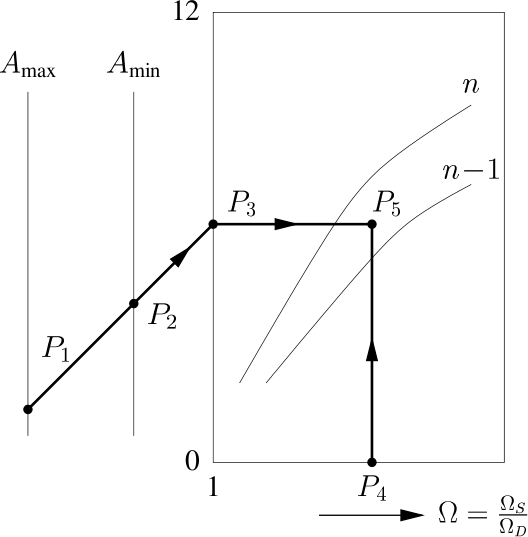
\includegraphics[width=6cm]{./images/filter-nomogramme.png}
	}
& \parbox{12cm}{
	\textbf{Oder mittels Formeln}\\
	$n_{\text{Butterworth}} \geq\frac{\log{\left[\displaystyle\frac{10^{A_{\min}/10}-1}
	{10^{A_{\max}/10}-1}\right]}} {2 \cdot \log{\left(\frac{\Omega_{S}}{\Omega_{D}}\right)}}$ \\ \\

	$n_{\text{Tschebyscheff}_{(\text{I,II})}} \geq\frac{{\rm Arcosh}\sqrt{\displaystyle\frac{10^{A_{\min}/10}-1}
	{10^{A_{\max}/10}-1}}}{{\rm Arcosh}\left({\Omega_{S}/\Omega_{D}}\right)}$ \\ \\

	$n_{\text{Cauer}} \geq\frac{K\left(\left( \frac{\Omega_D}{\Omega_S}\right)^2\right)
	K\left(1-\frac{10^{A_{\max}/10}-1}{10^{A_{\min}/10}-1}\right) } {K\left(1-\left(\frac{\Omega_D}
	{\Omega_S}\right)^2\right )K\left(\frac{10^{A_{\max}/10}-1}{10^{A_{\min}/10}-1} \right)},
	\text{mit}\quad
	K(k)=\int_0^{\frac{\pi}{2}}\frac{d\theta}{\sqrt{1-k\sin^2\theta}}$ \\ \\
	
	\textbf{Oder mit Matlab}\\
	\texttt{buttord, cheb1ord, cheb2ord, ellipord}	
	}
\end{tabular} \\ \\
\textbf{Grundsätzlich gilt (für gleiche Spezifikationen)} \quad
$n_{\text{Butterworth}}\geq n_{\text{Tschebyscheff}_{(\text{I,II})}}\geq n_{\text{Cauer}}$
\subsubsection{UTF bestimmen \& entnormieren}
Die UTF kann meist aus Tabellen herausgelesen werden und variiert je nach
Filtertyp. Die Entnormierung erfolgt durch Substitution von $S \longrightarrow
\displaystyle\frac{s}{\omega_{\text{3dB}}}$, wobei auch hier
$\omega_{\text{3dB}}$ je nach Filtertyp unterschiedlich berechnet wird.

\renewcommand{\arraystretch}{1.5}
\begin{tabular}{|p{6cm}|p{6cm}|p{6cm}|}
\hline
Butterworth \formelbuch{345}
	& Tschebyscheff I \formelbuch{349}
	& Kritisch gedämpfte Filter \formelbuch{347}\\
$\omega_{\text{3dB}}=\sqrt[2n]{\frac{1}{10^{A_{\max}/10}-1}}\cdot \omega_{D}$
	&
	$\omega_{\text{3dB}}=\cosh{\left[\left(\frac{1}{n}\right) {\rm
	Arcosh}\left(\frac{1}{e}\right)\right]} \cdot \omega_{D}$\newline
	Wobei $e = \sqrt{10^{A_{max}/10}-1}$
	& $\omega_{3\text{dB}}=\frac{\omega_D \cdot{\sqrt{2^{1/n}-1}}
	}{\sqrt{10^{\frac{A_{\text{max}}}{10\cdot n}}-1}}$ \\
\hline
Cauer \formelbuch{356}
	& Bessel \formelbuch{353}
	& \\
Keine Tabelle, \matlab{ellip, ellipap}
	& $\omega_{3\text{dB}}$ aus Abb. 7.93 \formelbuch{354}
	& \\
\hline
\end{tabular}
\renewcommand{\arraystretch}{1}


\subsubsection{LC-Tiefpass bestimmen \formelbuch{???,
420}}
\begin{tabular}{ll}
\parbox{10cm}{
	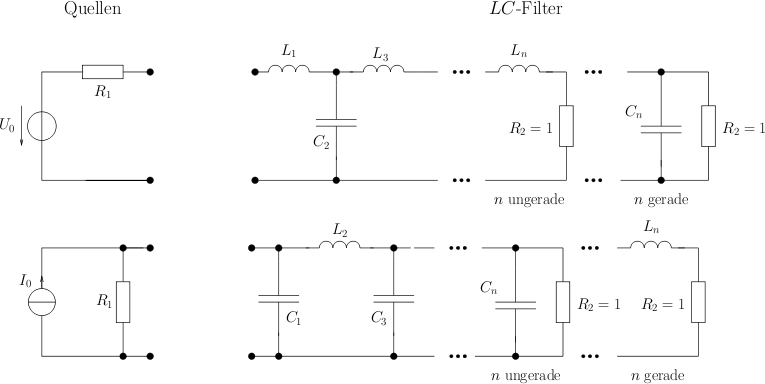
\includegraphics[width=10cm]{./images/filter-lc-realisation.png}
	}
& \parbox{8cm}{
	Die Struktur unterscheidet sich nicht zwischen den Filtertypen.\\
	Es ist zwischen Minimal-C (meistens) und Minimal-L-Netzwerken auszuwählen. \\
	\\
	Erläuterungen zu den Tabellen:
	\begin{itemize}
     \item Die Legende oben beschreibt die Stromquellenstruktur, die untere die
	Spannungsquellenstruktur.     
	\item Normierung auf $R_2 = 1$, folglich $R_1 =
	\frac{R_{\text{Quelle}}}{R_{\text{Last}}}$
    \end{itemize}
	}
\end{tabular}

\textbf{Tabellenindex} \\
\renewcommand{\arraystretch}{1.5}
\begin{tabular}{|p{5.5cm}|p{5.5cm}|p{6cm}|}
\hline
Butterworth \formelbuch{421}
	& Tschebyscheff I \formelbuch{424, 425}
	& Kritisch gedämpfte Filter \formelbuch{423}\\
\hline
Cauer \formelbuch{427, 428}
	& Bessel \formelbuch{422}
	& \\
\hline
\end{tabular}
\renewcommand{\arraystretch}{1} \\

\textbf{Entnormierung}\\
Aus den Tabellen gelesene Werte werden im folgenden als $C'$ bzw. $L'$
bezeichnet.\\ 
$C = \frac{C'}{\omega_{\text{3dB}} R_{\text{Last}}}$ \qquad $L = \frac{L'
R_{\text{Last}}}{\omega_{\text{3dB}}}$


\begin{tabular}{ll}
\parbox{11.5cm}{
	\subsubsection{Bauteiltransformation zum gewünschten Filter \formelbuch{386}}
	\renewcommand{\arraystretch}{1.5}
	\begin{tabular}{|p{2cm}|p{7.5cm}|}
	\hline
	Tiefpass-Hochpass
		& \parbox{7cm}{
		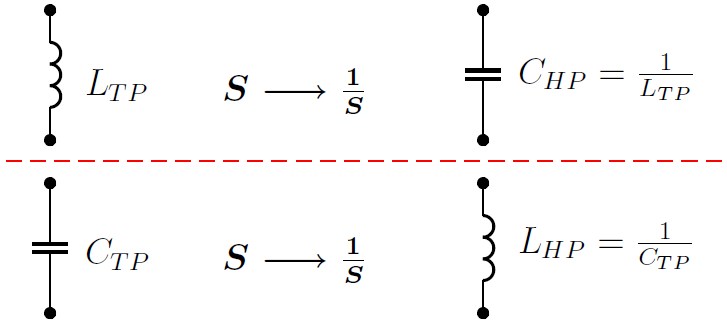
\includegraphics[width=7cm]{./images/filter-bauteile-tp-hp.png}}
		\\
	\hline
	Tiefpass-Bandpass 
		& \parbox{7cm}{
		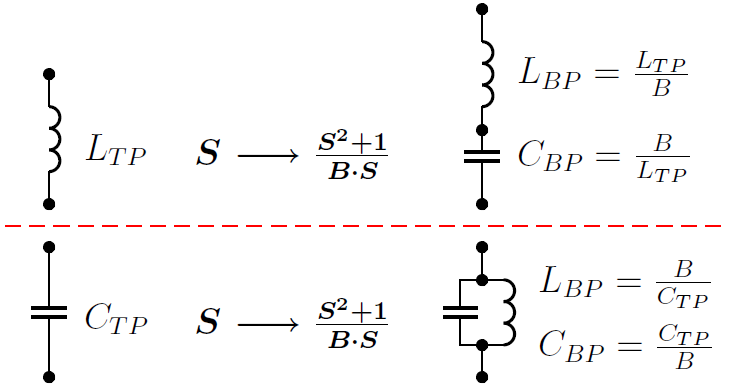
\includegraphics[width=7cm]{./images/filter-bauteile-tp-bp.png}}
		\\
	\hline
	Tiefpass-Bandsperre
		& \parbox{7cm}{
		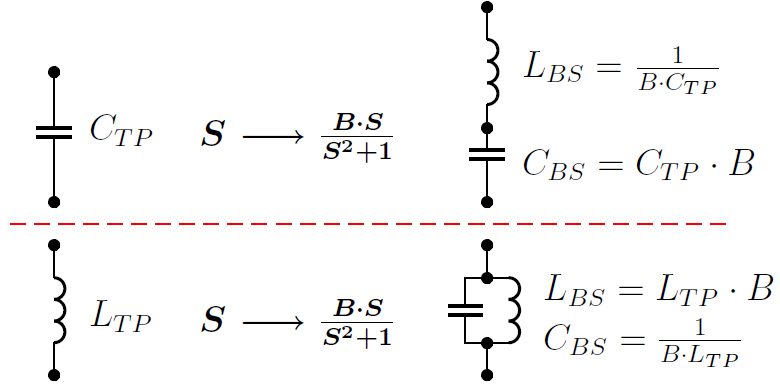
\includegraphics[width=7cm]{./images/filter-bauteile-tp-bs.png}}
		\\
	\hline
	\end{tabular}
	\renewcommand{\arraystretch}{1}
	}
& \parbox{7cm}{
	\subsection{Kaskadierung von Filtern}
	Wenn mehrere Filter kaskadiert werden, ändern sich die Spezifikationen wie in
	folgendem Beispiel:\\
	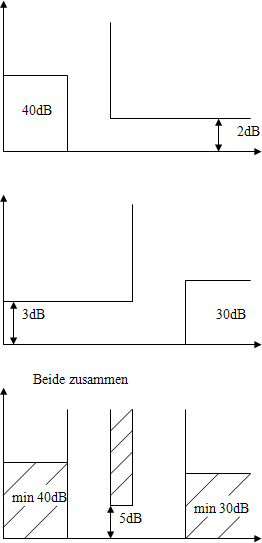
\includegraphics[width=4cm]{./images/filter-kaskadierung.png}
	}
\end{tabular}



\newpage
\subsection{Vergleich der Approximationsarten}
\scriptsize
\begin{center}
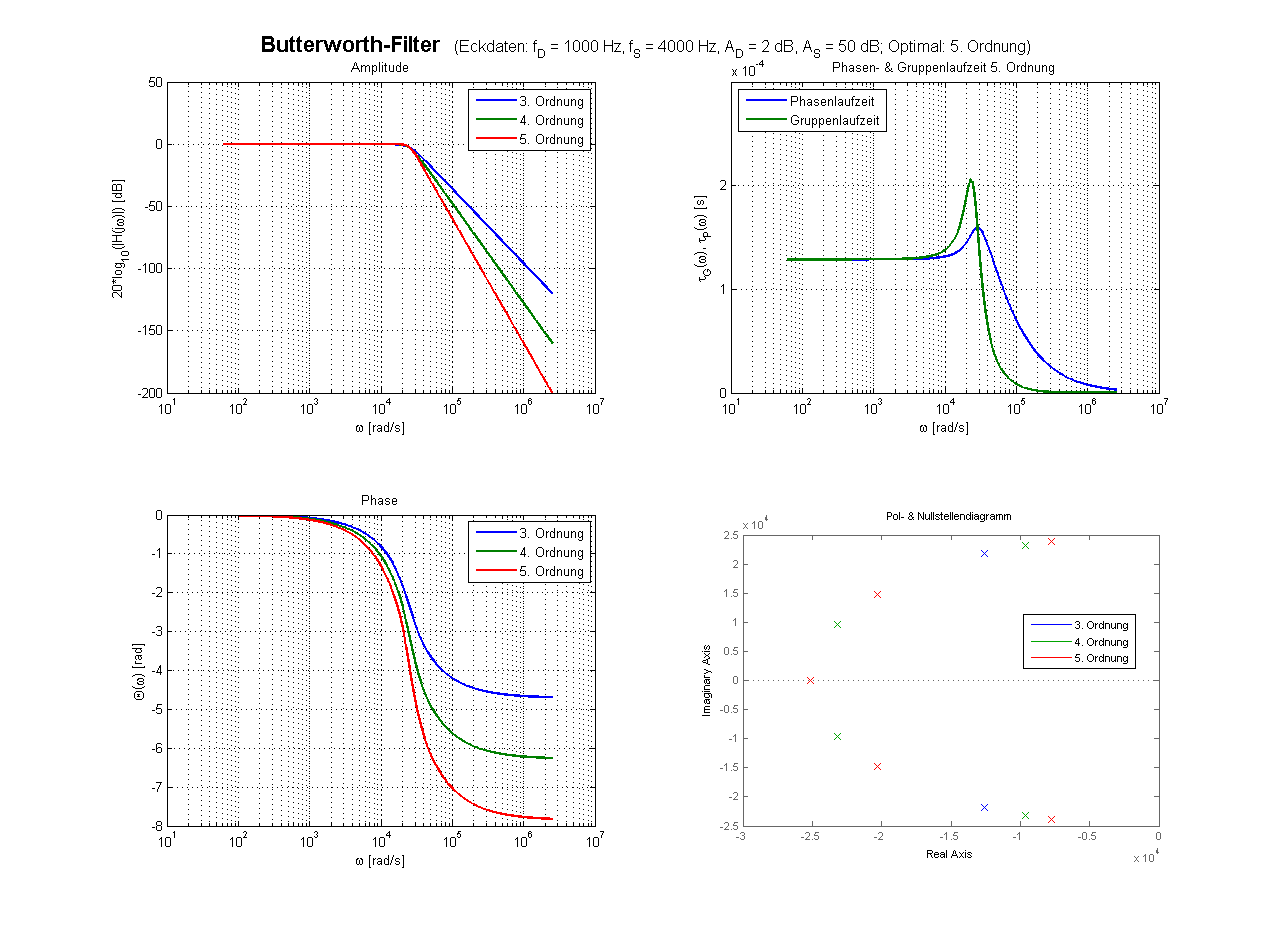
\includegraphics[height=11.5cm]{./images/filter-butterworth.png}
\\Butterworth-Filter mit UTF $H(s) = \frac{1.003e022}{s^5 + 8.133e004 s^4 +
3.307e009 s^3 + 8.312e013 s^2 + 1.291e018 s + 1.003e022}$ 
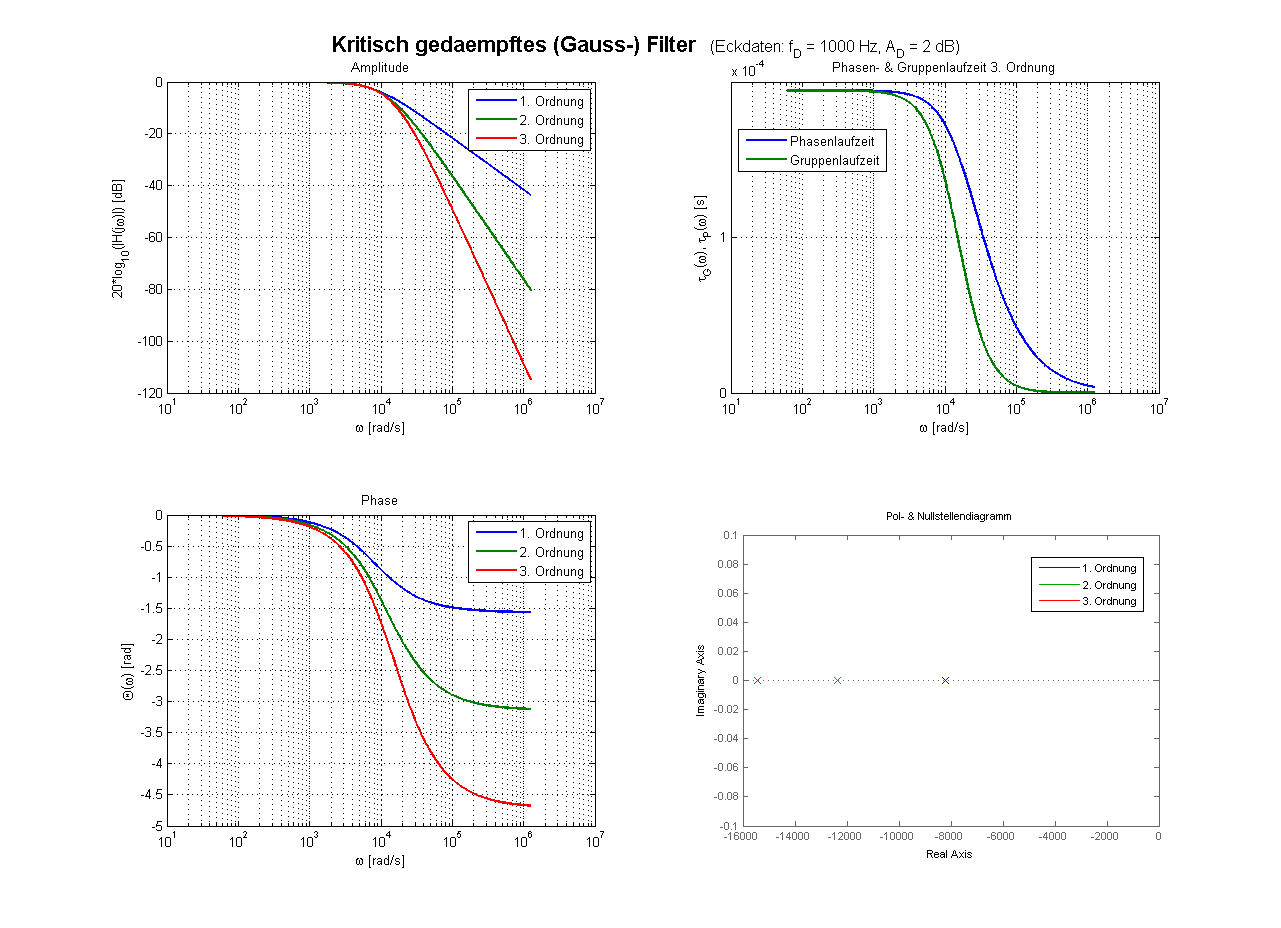
\includegraphics[height=11.5cm]{./images/filter-gauss.png} \\Kritisch gedämpftes
Filter mit UTF $H(s) = \frac{1}{2.724e-013 s^3 + 1.261e-008 s^2 + 0.0001945 s +
1}$ 
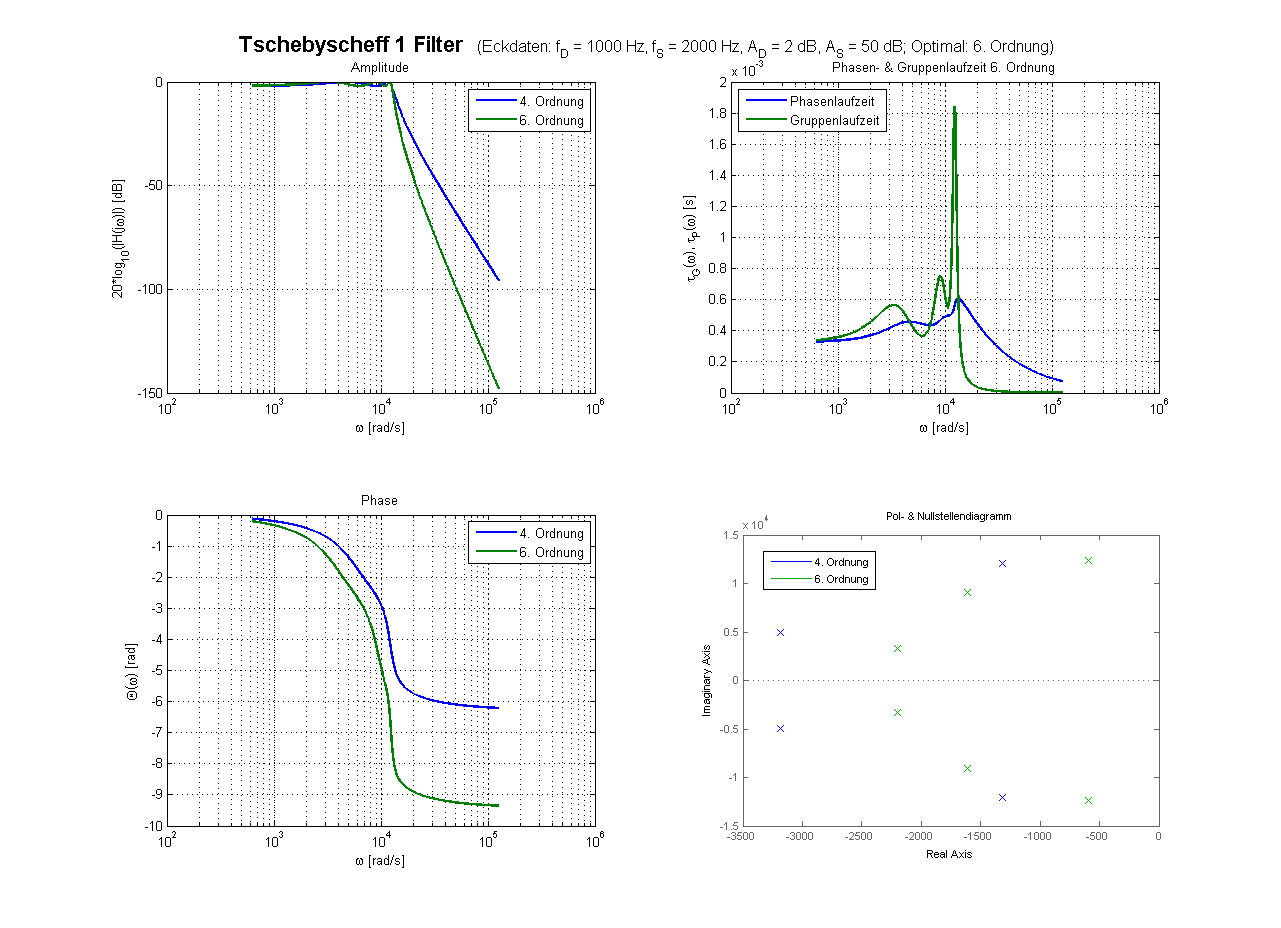
\includegraphics[height=12cm]{./images/filter-tschebyscheff1.png} \\Tschebyscheff-I-Filter mit UTF $H(s)
= \frac{1.609e023}{s^6 + 8812 s^5 + 2.757e008 s^4 + 1.721e012 s^3 + 1.924e016
s^2 + 6.589e019 s + 2.026e023}$ 
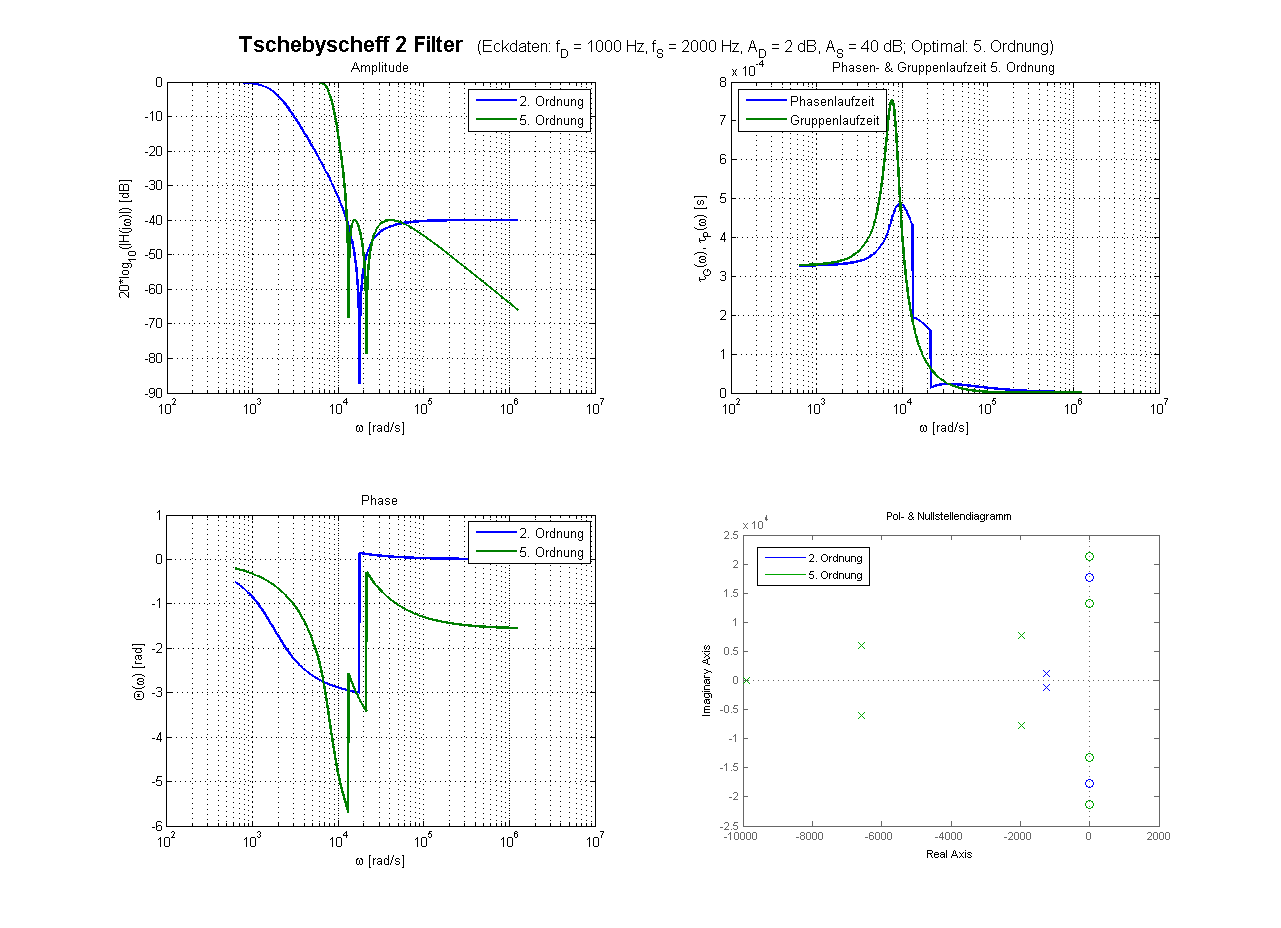
\includegraphics[height=12cm]{./images/filter-tschebyscheff2.png} \\Tschebyscheff-II-Filter mit UTF
$H(s) = \frac{628.3 s^4 + 1.081e-009 s^3 + 3.969e011 s^2 + 1.975 s +
5.014e019}{s^5 + 2.701e004 s^4 + 3.645e008 s^3 + 3.076e012 s^2 + 1.639e016 s + 5.014e019}$
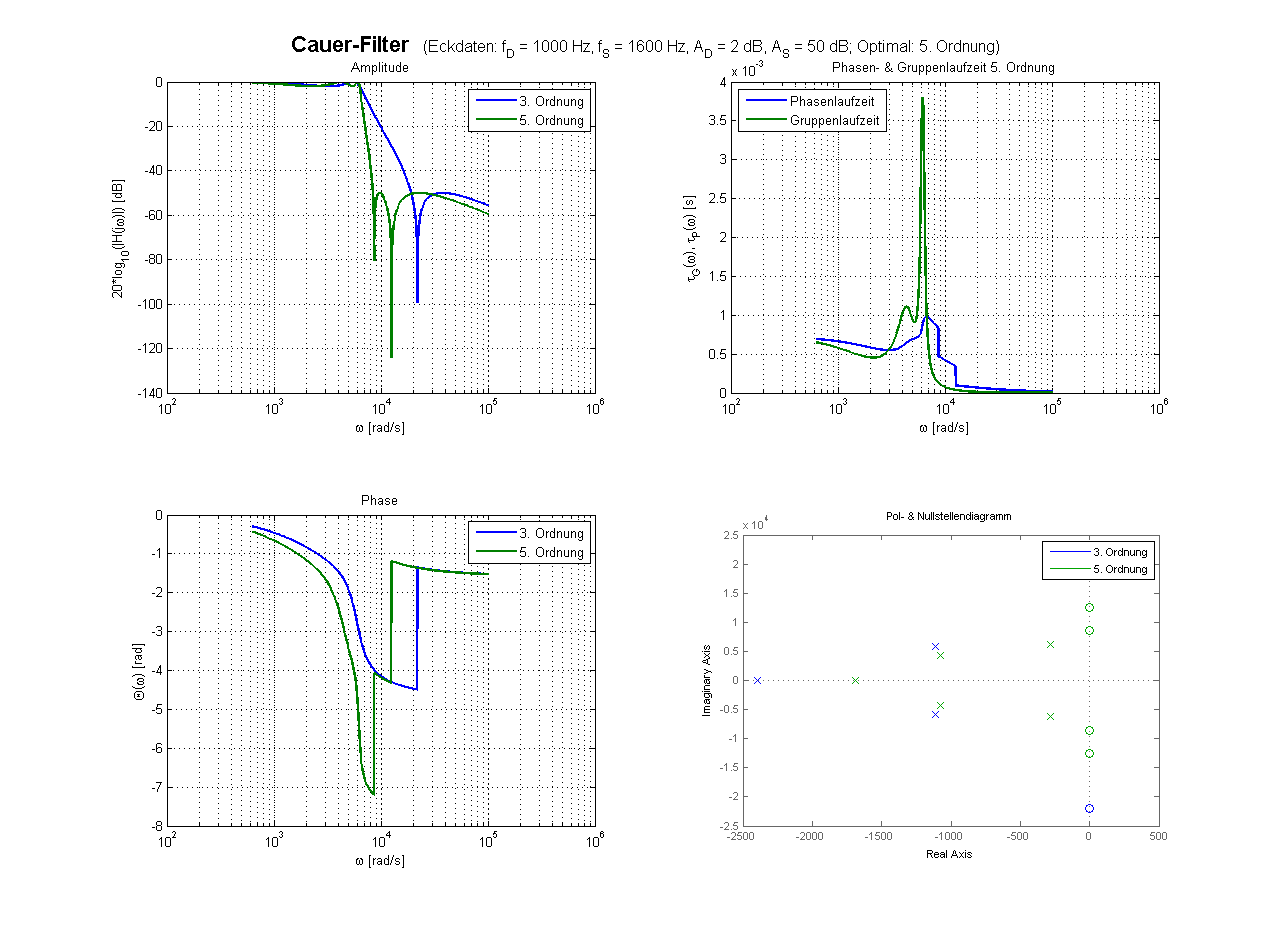
\includegraphics[height=12cm]{./images/filter-cauer.png} \\Cauer-Filter mit UTF
$H(s) = \frac{108.8 s^4 - 6.596e-010 s^3 + 2.538e010 s^2 - 0.08009 s + 1.29e018}{s^5 + 4398 s^4 + 6.408e007 s^3 + 1.939e011 s^2 + 9.227e014 s + 1.29e018}$
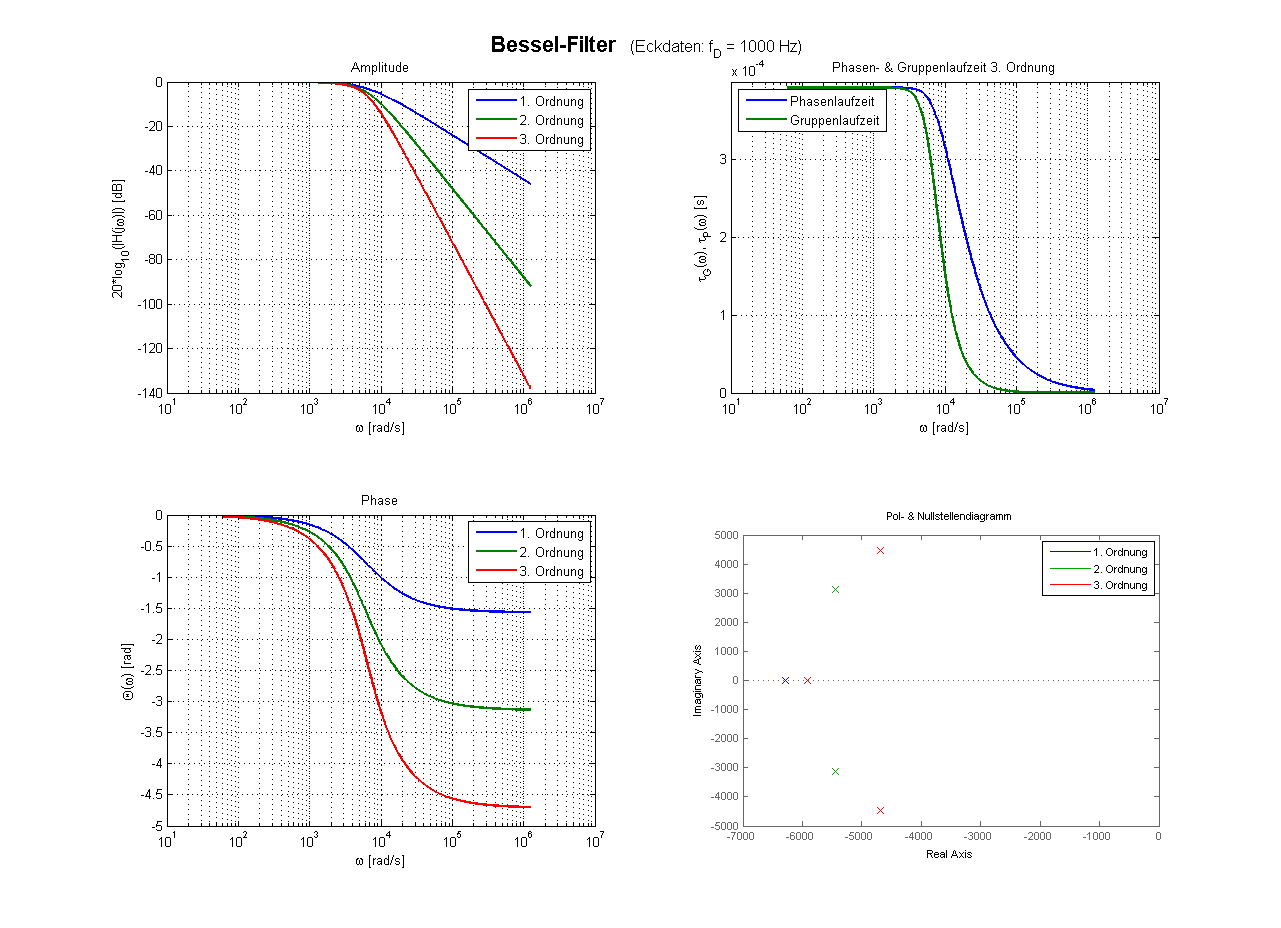
\includegraphics[height=12cm]{./images/filter-bessel.png} \\Bessel-Filter mit UTF $H(s) =
 \frac{2.481e011}{s^3 + 1.529e004 s^2 + 9.736e007 s + 2.481e011}$
\end{center}


